\chapter{Approach}
To measure the RSSI of each link all the nodes need to send messages. Since two nodes sending a message at the same time will distort the RSSI measurements we need to make sure that only one node sends a message to a given point in time. One approach to archive this is the timeslot based method explained in Chapter 2.3. This method however includes an error inside its timeslots, resulting in a small delay between messages.
To eliminate the delay timeslots bring along a different approach is suggested in this thesis which is based on predefined predecessors for each node. Based on this a node will be able to send a message directly after receiving a message from its predecessor and at the same time making sure that only one node sends at a given point in time.

\section{General Structure}

The system consists of a base station with high processing power and a lot of memory and multiple distributed low power nodes. One of the nodes is the sink which is directly connected to the base station. The nodes are able to communicate with each other via radio, however not every node can hear all the other nodes. This structure is represented by Figure 3.1 (a). The fact that not every node is able to hear all the other nodes makes it a challenge to collect data from the network and to create a fitting schedule that defines predecessors for all the nodes inside the network. To be able to do so a first calibration phase needs to create paths from every node to the sink and collect information about the connections between nodes. Then the information about the connections need to be collected at the sink and send to the base station in a collection phase. When the base station received all the information it can create the schedule. After that the base station needs to send the schedule to the sink that starts spreading it inside the network. Is the schedule spread and all the nodes know when to send their messages the sampling of the RSSI can start. Therefore messages are send according to the, in the schedule defined, predecessors to measure the RSSI. When the schedule is completed another collection of the data is needed to gather the measured RSSI at the base station for further processing. If the collection is done the system can start sampling again and then again collect the data until the system is stopped. This process is schown in Figure 3.1 (b).    

\begin{figure}[htbp]
	\centering
	\begin{subfigure}[t]{0.4\textwidth}
		\centering
    		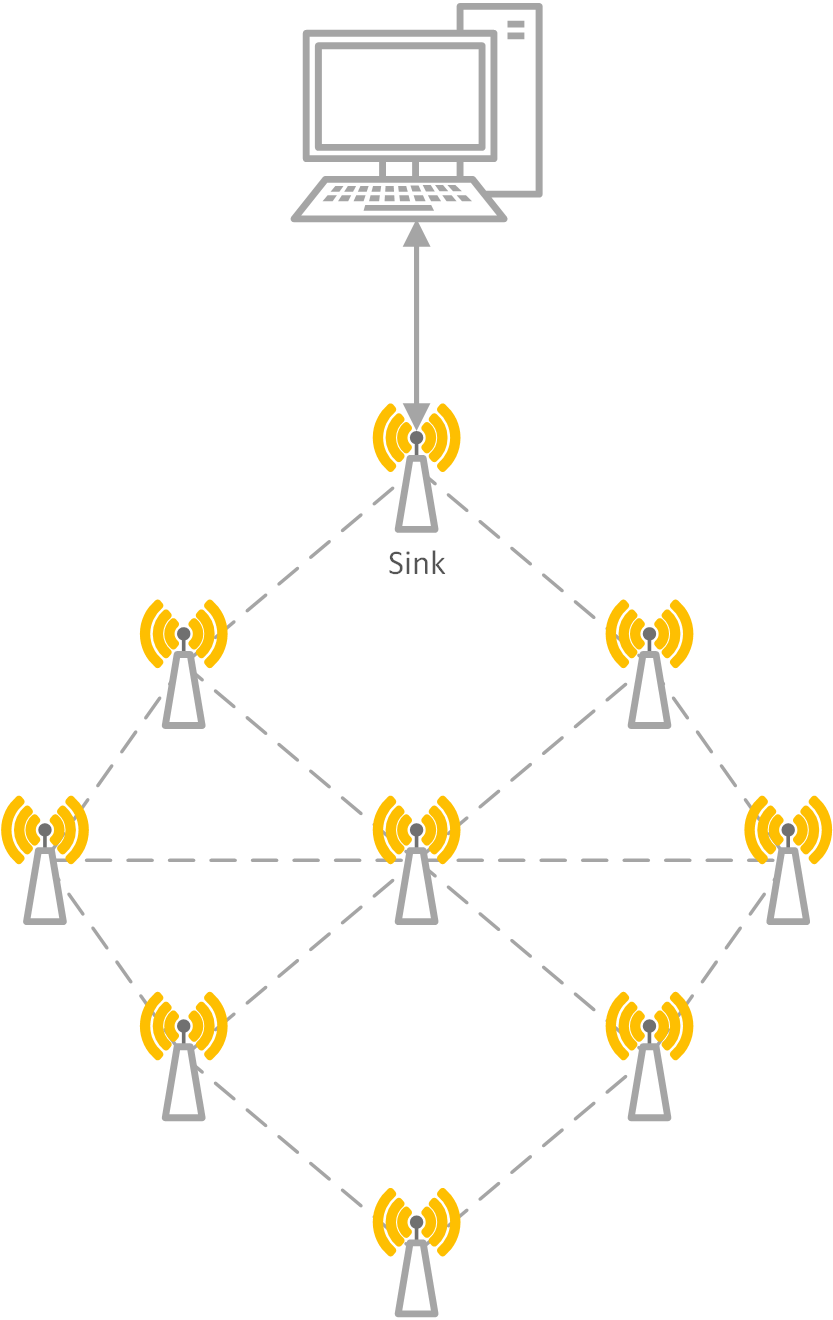
\includegraphics[scale=0.7]{content/images/Architecture}
   	 	\caption{The physical architecture of the system}
    	\label{fig:density}
    \end{subfigure}
    \quad
    \quad
    \quad
    \begin{subfigure}[t]{0.4\textwidth}
		\centering         
        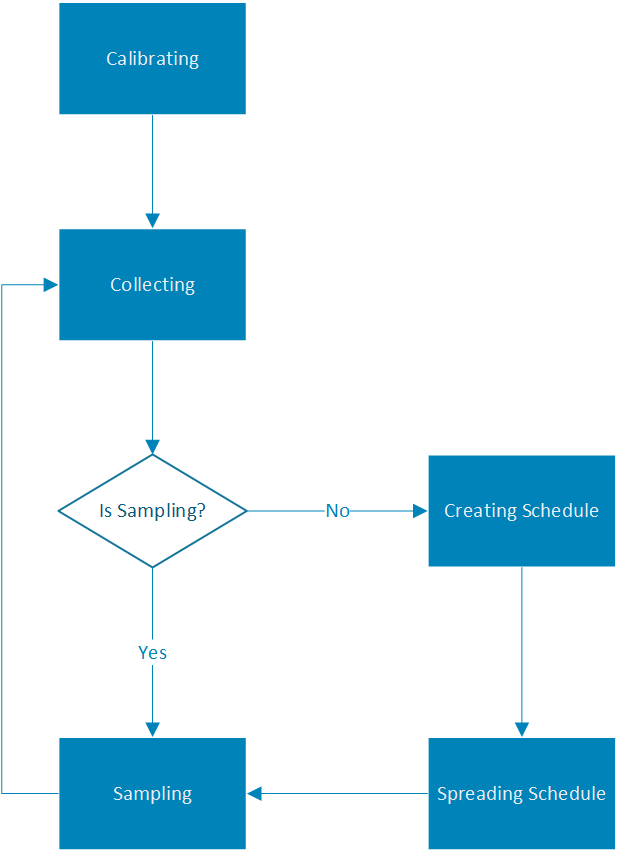
\includegraphics[scale=0.7]{content/images/GeneralAproachM}
        \caption{The general processes and the order in which they are executed}
        \label{fig:link}
    \end{subfigure}
    \caption{}
\end{figure}

\section{Base Station}
Since creating the schedule and storing and processing the data need a lot of processing power and storage a base station that fulfils these requirements is needed. This base station needs to be connected to the sink so it can receive the collected data to process it. It also needs to be able to send data to the sink, so the schedule can be spread inside the network.    
\section{Calibration}
To find out the existing links between nodes the calibration phase is needed. Moreover this phase will establish paths from each node to the sink. On these paths data can be send to gather it at the sink. To do so each node will just start sending messages without specific pattern. These message include a value that describes the quality of the path that node has to the sink and the next hop of the node which is the next node along the path. When a node receives a message it will add the sending node into a neighbourlist including the data bout its next hop. By including the data of the next hop we make sure that the path is known into both directions. Then it will compare its own path quality with the received one. If the received path quality is higher the path of the node will be adjusted. It will set its own next hop to the the sending node and set its new path quality accordingly. When the calibration is finished the whole network can now also be seen as a tree where the connection between the nodes is given through the path with the sink as the root where each node knows its parent and its children.
\subsection{Path Quality}
The path quality is a mixture of the amount of nodes a path has and the signal strength between these nodes. To calculate it the signal strength is divided into an interval. Each interval gets a value. If a node receives a message it will assign the value according to the received signal strength and the defined interval and add this value to the path quality given inside the message. 


This chapter is not really good...
\section{Collection}

\begin{figure}[htbp]
	\centering
	\begin{subfigure}[t]{0.4\textwidth}
		\centering
    		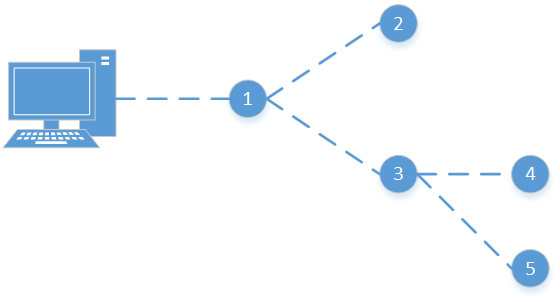
\includegraphics[scale=0.6]{content/images/Collection/Part0}
   	 	\caption{At the beginning all the nodes are unmarked and still have data to send}
    	\label{fig:density}
    \end{subfigure}
    \quad
    \quad	
	\begin{subfigure}[t]{0.4\textwidth}
		\centering
    		\includegraphics[scale=0.6]{content/images/Collection/Part1}
   	 	\caption{Node 1 sends the first request to node 2}
    	\label{fig:density}
    \end{subfigure}
    \quad
    \quad
    \begin{subfigure}[t]{0.4\textwidth}
		\centering         
        \includegraphics[scale=0.6]{content/images/Collection/Part2}
        \caption{Node 2 does not have any children so it sends its data and gets marked}
        \label{fig:link}
    \end{subfigure}
    \quad
    \quad
    \begin{subfigure}[t]{0.4\textwidth}
		\centering         
        \includegraphics[scale=0.6]{content/images/Collection/Part3}
        \caption{Now node 2 is marked so node 1 sends a request to node 3, which forwards it to node 4}
        \label{fig:link}
    \end{subfigure}
    \quad
    \quad
    \begin{subfigure}[t]{0.4\textwidth}
		\centering         
        \includegraphics[scale=0.6]{content/images/Collection/Part4}
        \caption{Node 4 does not have any children so it sends its data and gets marked}
        \label{fig:link}
    \end{subfigure}
    \quad
    \quad
    \begin{subfigure}[t]{0.4\textwidth}
		\centering         
        \includegraphics[scale=0.6]{content/images/Collection/Part5}
        \caption{Node 3 is still not marked so node 1 sends a request to it. Node 4 is marked so node 3 forwards the request to node 5}
        \label{fig:link}
    \end{subfigure}
    \quad
    \quad
    \begin{subfigure}[t]{0.4\textwidth}
		\centering         
        \includegraphics[scale=0.6]{content/images/Collection/Part6}
        \caption{Node 4 does not have any children so it sends its data and gets marked}
        \label{fig:link}
    \end{subfigure}
    \quad
    \quad
    \begin{subfigure}[t]{0.4\textwidth}
		\centering         
        \includegraphics[scale=0.6]{content/images/Collection/Part7}
        \caption{Node 3 is still not marked so node 1 sends a request to it}
        \label{fig:link}
    \end{subfigure}
    \quad
    \quad
    \begin{subfigure}[t]{0.4\textwidth}
		\centering         
        \includegraphics[scale=0.6]{content/images/Collection/Part8}
        \caption{All the children of node 3 are marked so it starts sending its data and gets marked itself}
        \label{fig:link}
    \end{subfigure}
    \quad
    \quad
    \begin{subfigure}[t]{0.4\textwidth}
		\centering         
        \includegraphics[scale=0.6]{content/images/Collection/Part9}
        \caption{Now all the children of node 1 are marked and it can send its own data to the base station and gets marked}
        \label{fig:link}
    \end{subfigure}
    \caption{This is an example for the collection. REQ means request and DAT Sx stands for data from source x}
\end{figure}

To collect the data from the network we make use of the created paths and their tree structure. The sink will send a request to one of its children. The child receiving that request will check if it has any children himself and if that is the case it will forward the request to one of them. When the request reaches a node without any children it will send his data to his parent which will forward the data his parent, until the data reach the sink who will forward them to the base station. Every node that receives the data will mark the source of that data as done. When the sink send the received data to the sink it will send a new request to one of its children that has not been marked as done. That child will again forward that request to a child that has not been mark as done. If the request reaches a node that has no children or every child has been marked as done it will send its own data. This process will be repeated until the sink does not have any more children that are not marked as done left. Then the sink can send its own data to the base station and finish the collection. All the nodes now need to unmark all the other nodes, so another collection is possible. In Figure 3.2 an example for this process is given. The Figure shows a wireless sensor network represented by the nodes and the, in the calibration created, paths to the sink. Note that the nodes could also have other connections between each other.

\section{Creating the Schedule}
Creating a schedule is a quite challenging task since we need an algorithm that visits every node in a graph at least one time and starts and ends at the same node. The optimal schedule would be a Hamilton-Circle that is one circle inside a graph that visits each node exactly once. To Figure out if there is a Hamilton-Circle existing there is however only the way to bruteforce all the possible combinations. This is highly inefficient and possibly we do not even get a result at the end. Therefore this thesis suggests a simple method that makes sure every node gets visited at least once and the path starts and ends at the same node. This method however is not able to create a optimal path and could be improved quite a lot.

\subsection{Rooted Circles}
\begin{figure}[htbp]
	\centering
	\begin{subfigure}[t]{0.4\textwidth}
		\centering
    		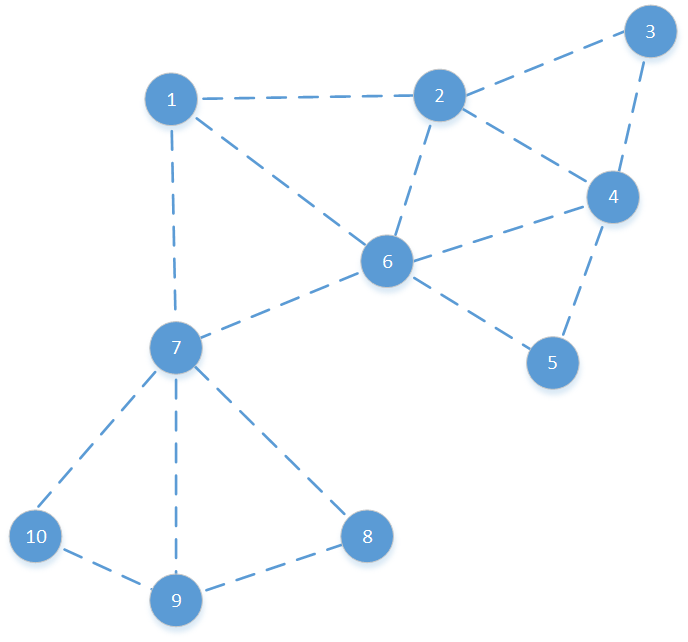
\includegraphics[scale=0.6]{content/images/Schedule/Network}
   	 	\caption{The example network with all its connections between nodes}
    	\label{fig:density}
    \end{subfigure}
    \quad
    \quad
    \begin{subfigure}[t]{0.4\textwidth}
		\centering         
        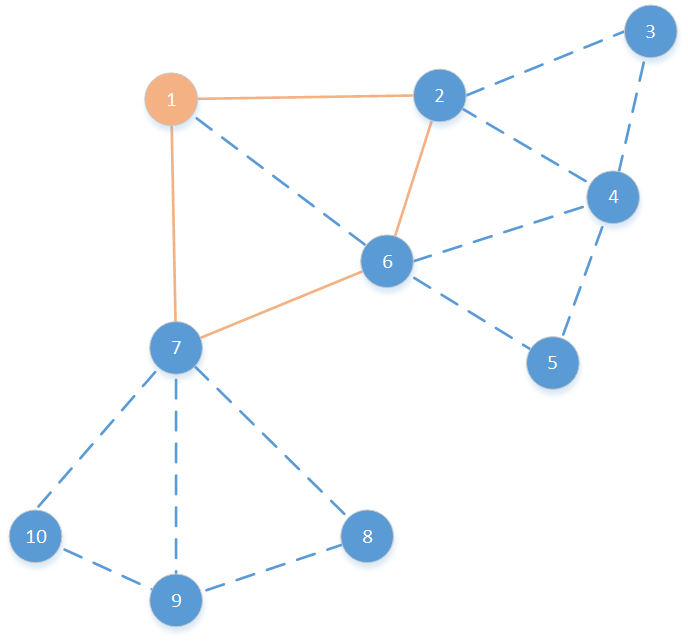
\includegraphics[scale=0.6]{content/images/Schedule/RootedCircle}
        \caption{Example for a rooted circle with node 1 as the root}
        \label{fig:link}
    \end{subfigure}
    \caption{A rooted circle inside a example network}
\end{figure}

The suggested method is based on smaller circles inside the graph. These circles will have a root node that is the entrance and the end point of the circle. All the nodes inside this circle will be in range of the root of the circle. These circles will be called rooted circles. In Figure 3.3 (b) such a rooted circle is represented inside the network represented by Figure 3.3 (a). To create a rooted circle one node needs to be chosen as the root. Then the root will take one node from its neighbour table and chose it as it as the second node in the circle.  Than the second node will look into its neighbour table and chose a node that has the root node inside its neighbour table. The chosen node will do the same and the process will be repeated until a node does not have a neighbour that has the root as a neighbour. Then the circle will be closed and the path goes to the root. When we look at the example in Figure 3.3 (b) this means node 1 was chosen as the root. Then node 2 was picked as the second node in the circle. Node 2 has multiple neighbours but only one of them, node 6, has the root node 1 as a neighbour. This means node 6 is chosen as the next node in the circle. Node 6 now has node 2 and node 7 as neighbours that also have the root as a neighbour, however node 2 is already inside the circle so node 7 is chosen as the next node. Node 7 now has no more neighbours that have the root as a neighbour and the circle is closed.

\subsection{Creating a Full Schedule}
\begin{figure}[htbp]
	\centering         
    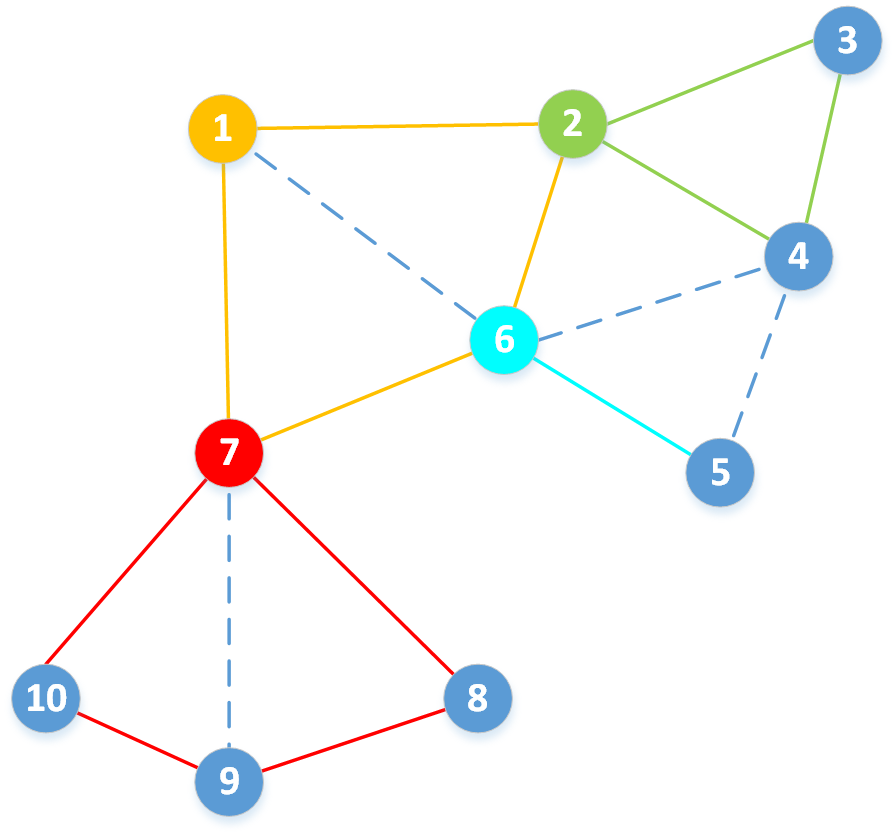
\includegraphics[scale=0.6]{content/images/Schedule/FullSchedule}
    \label{fig:link}
    \caption{Full schedule for the example network of figure 3.3 (a). The order in which the nodes send their messages would be: 1 2 3 4 2 6 5 6 7 8 9 10 7 1.}
\end{figure} 
We now want to fill the whole graph with rooted circles. Therefore we will chose the sink as the first root and create a rooted circle around it. When the circle is done we will go through all the nodes of the circle and, if possible, create rooted circle around them as well. Then we do the same for all the new circles until every node once was suggested as a root. When creating new circles it is not possible to choose a node already inside another circle to be part in the new circle. In Figure 3.4 the network from Figure 3.3 (a) is fully covered by rooted circles. The first circle created was the on that has node 1 as a root. Then all the nodes inside that circle where chosen as new roots to create new rooted circles. The first thing one could notice is that the circle with the root 6 only has one other node and does not really forms a circle. This happens if the circle is closed directly after the second node, following the root, is chosen because there are no more neighbours left that also have the root as a neighbour. When running the schedule this means a message would be send from node 6 to node 5 and then from node 5 back to node 6. Also note that in theory there is a bigger rooted circle possible with the root 6 when node 4 would be included, but node 2 created its rooted circle first and included node 4 and therefore blocked it for rooted circles created at a later point in time. In Listing 3.1 you will find pseudocode that represents an algorithm to cover a whole graph with rooted circles.

\begin{document}
\lstset{caption={Pseudocode that covers a graph with rooted circles}}
\begin{lstlisting}
RootedCircle createRootedCircle(Node root) {
	Node node = getNextForCircle(root, root)	

	if(node != null) {
		RootedCircle rootedCircle = new rootedCircle(root)
		rootedCircle.addNode(node)

		while((node = getNextForCircle(root, node)) != null)
			rootedCircle.add(node)

		return rootedCircle
	} else {
		return null
	}
}

Node getNextForCircle(Node root, Node neighbour) {
	for each (Node node in root.getNeighbourList)	
		if(node.isNeighbourOf(neighbour) and not node.isPartOfACircle())
			return node
	return null
}

List<RootedCircle> coverGraphWithRootedCircles(Node firstRoot) {
	List<RootedCircle> circleList = new List<RootedCircle()>
	
	circleList.add(createRootedCircle(firstRoot))

	for each (RootedCircle circle in circleList) {
		for each (Node node in circle) {
			RootedCircle newCircle = createRootedCircle(node)
			if(newCircle != null)
				circleList.add(newCircle);
		}
	}
}
\end{lstlisting}
\end{document}

\section{Spreading the Schedule}
To spread the schedule we will again make use of the tree structure of the created path. When the sink received the schedule from the control point it will forward it to its first child. The child will forward it to one of his children and so on. When a node that received the schedule has no more children it will send the schedule back to its parent. The parent receiving the schedule will now forward the schedule to its next child. If a parent received the schedule back from all its children it will forward it to its own parent. In Figure 3.5 an example for this process is given. The Figure shows a wireless sensor network represented by the nodes and the, in the calibration created, paths to the sink. Note that the nodes could also have other connections between each other. When you look at the example you can see that already in Figure 3.5 (g) the schedule is received by all the nodes but still there are messages send that could seem useless at this point. However at this point in time we do not know if the sink has any more children that did not receive the schedule jet. Therefore the schedule needs to travel all the way back to the sink. Only at the moment the schedule reaches the sink and the sink does not have any more children left that need to receive the schedule we know for sure that the schedule is fully spread.

\begin{figure}[htbp]
	\centering
	\begin{subfigure}[t]{0.4\textwidth}
		\centering
    		\includegraphics[scale=0.6]{content/images/ScheduleSpreading/Part1}
   	 	\caption{The base station sends the schedule to node 1.}
    	\label{fig:density}
    \end{subfigure}
    \quad
    \quad
    \begin{subfigure}[t]{0.4\textwidth}
		\centering         
        \includegraphics[scale=0.6]{content/images/ScheduleSpreading/Part2}
        \caption{Node 1 forwards the schedule to node 2}
        \label{fig:link}
    \end{subfigure}
    \quad
    \quad
    \begin{subfigure}[t]{0.4\textwidth}
		\centering         
        \includegraphics[scale=0.6]{content/images/ScheduleSpreading/Part3}
        \caption{Node 2 does not have any children and sends the schedule to its parent node 1}
        \label{fig:link}
    \end{subfigure}
    \quad
    \quad
    \begin{subfigure}[t]{0.4\textwidth}
		\centering         
        \includegraphics[scale=0.6]{content/images/ScheduleSpreading/Part4}
        \caption{Node 2 is now marked so node 1 will forward the schedule to node 3}
        \label{fig:link}
    \end{subfigure}
    \quad
    \quad
    \begin{subfigure}[t]{0.4\textwidth}
		\centering         
        \includegraphics[scale=0.6]{content/images/ScheduleSpreading/Part5}
        \caption{Node 3 forwards the schedule to node 4}
        \label{fig:link}
    \end{subfigure}
    \quad
    \quad
    \begin{subfigure}[t]{0.4\textwidth}
		\centering         
        \includegraphics[scale=0.6]{content/images/ScheduleSpreading/Part6}
        \caption{Node 4 does not have any children and sends the schedule to its parent node 3}
        \label{fig:link}
    \end{subfigure}
    \quad
    \quad
    \begin{subfigure}[t]{0.4\textwidth}
		\centering         
        \includegraphics[scale=0.6]{content/images/ScheduleSpreading/Part7}
        \caption{Node 3 has still node 5 as an unmarked child and forwards the schedule to it}
        \label{fig:link}
    \end{subfigure}
    \quad
    \quad
    \begin{subfigure}[t]{0.4\textwidth}
		\centering         
        \includegraphics[scale=0.6]{content/images/ScheduleSpreading/Part8}
        \caption{Node 5 does not have any children and sends the schedule to its parent node 3}
        \label{fig:link}
    \end{subfigure}
    \quad
    \quad
    \begin{subfigure}[t]{0.4\textwidth}
		\centering
    		\includegraphics[scale=0.6]{content/images/ScheduleSpreading/Part9}
   	 	\caption{Node 3 has no more unmarked children and sends the schedule to its parent node 1}
    	\label{fig:density}
    \end{subfigure}
    \quad
    \quad	
    \begin{subfigure}[t]{0.4\textwidth}
		\centering         
        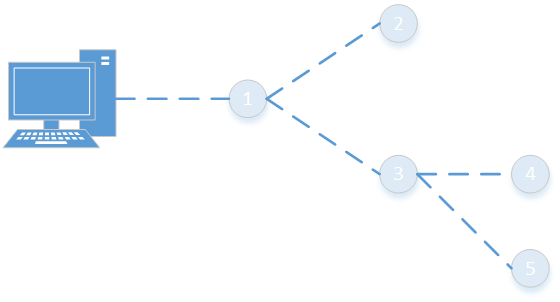
\includegraphics[scale=0.6]{content/images/ScheduleSpreading/Part10}
        \caption{Since node 1 does not have any more unmarked children the schedule is now fully spread inside the network}
        \label{fig:link}
    \end{subfigure}
    \caption{This is an example for a path a schedule message takes to be spread inside the network}
\end{figure}

\section{Sampling}
When all the nodes received the schedule it is possible to sample the received signal strength by sending messages according to it. Therefore the sink will start sending a message. When its successor receives the message it can send its message and so on until the last message was send and the sampled data can be collected. However we need to take into account that one node could appear multiple times inside the schedule, meaning a node could have multiple predecessors and successors. Therefore we need to include the successor of the sending node inside the message so a receiving node can see if he is the correct successor at that moment. 
\subsection{Message Drops}
A problem of the proposed method are message drops. If a successor does not receive the message of its predecessor the whole system would stop. Here a similar technique timeslots use comes in handy. For this method every node needs to know the whole schedule and not only its own predecessors and successors. Then whenever a node receives a message it can look up how many nodes need to send between the node that just send and itself. Than the amount of sending nodes is multiplied by a maximal time a node needs to send. The result is the time after the node can send its own message without receiving a message from its predecessor. Again we need to take into account that a node can appear multiple times in the schedule. Therefore after a node send a message it needs to calculate the maximal time until it will send the next message.
